\documentclass[11pt,a4paper,twoside]{article}

\usepackage{a4wide}
\usepackage{moreverb}
\usepackage{graphicx}
\usepackage{wrapfig}
\usepackage{expdlist}
\usepackage{svn}
\usepackage{fancyhdr}
\usepackage{extramarks}
\usepackage{color}
\usepackage[colorlinks=true,urlcolor=blue,linkcolor=blue]{hyperref}
\usepackage{ifthen}

\pagestyle{fancy}
\renewcommand{\sectionmark}[1]{\markboth{\thesection.\ #1}{}}

% Begin new paragraphs without indentation but vertical space.
\setlength{\parindent}{0pt}
\setlength{\parskip}{1.5ex plus 0.5ex minus 0.2ex}

\newcommand{\DOMjudge}{\textsc{DOM}judge }

% Display commands, arguments, etc. in texttt font and don't break those.
\newcommand{\cmd}[1]{\mbox{\texttt{#1}}}

% Only show text if the submitclient is configured
\newcommand{\ifcmdsubmit}[1]{\ifthenelse{\equal{\SUBMITCLIENTENABLED}{yes}}{#1}{}}

% Our titlepage, should be called at start of team manual document
% Argument list:
% #1 - DOMjudge version
% #2 - Document revision
% #3 - Last modified date
% #4 - Generated date
% Also define the following words for language overrides:
\newcommand{\versionrevison}{Version/revision}
\newcommand{\lastmodified}{Last modified}
\newcommand{\generated}{Generated}
\makeatletter
\newcommand{\titlestuff}[4]{%

  \thispagestyle{plain}
  \vspace*{-3cm}
  \parbox[t]{\linewidth}{%
    \begin{wrapfigure}[1]{r}{2cm}
      \vspace*{-1cm}\hfill
      \includegraphics[height=4cm]{../logos/DOMjudgelogo.pdf}
    \end{wrapfigure}
    {\fontfamily{phv}\fontseries{b}\fontsize{26pt}{28pt}\selectfont \@title \par}
  }
  \vskip 2cm

  % Setup fancy headers/footers (here because we need SVN stuff defined)
  \def\setupfancystuff{%
    \fancyhead{}
    \fancyfoot{}
    \fancyfoot[RO,LE]{\thepage}
    \fancyfoot[LO,RE]{%
      \color[gray]{0.5}\vspace{-0.3cm}
      \begin{tabular}{ll}
        \versionrevison: & #1 / #2 \\
        \lastmodified:   & #3 \\
        \generated:      & #4 \\
      \end{tabular}
    }
  }

  % First for fancy page style:
  \setupfancystuff
  \fancyhead[RO,LE]{\slshape \firstleftmark}

  % No headers for plain page style (titlepage):
  \fancypagestyle{plain}{%
    \setupfancystuff
    \renewcommand{\headrulewidth}{0pt}
  }
}
\makeatother


\usepackage[english]{babel}

% For inclusion of the correct date (last modified) and revision.
% Use the \SVN command to get language dependent formatting of the
% date. We need to do some %/$ comment character magic to satisfy both
% TeX and 'git log' format string formatting both with and without
% expansion of the $Format$ keyword below with 'git archive'.
\SVN $Date: 1900-01-01 00:00:00 +0000 $
\SVN $Rev: unpublished $
% $Format:
%n\SVN %x24Date: %ai %x24$
% $Format:
%n\SVN %x24Rev: %h %x24$

\title{\DOMjudge team manual}

\hypersetup{
	pdftitle={DOMjudge team manual},
	pdfauthor={DOMjudge Developers: domjudge-devel at domjudge.org},
	pdfsubject={Instruction for teams using the interface of the DOMjudge jury system during a programming contest},
	pdfkeywords={DOMjudge,manual,team,judge,jury,programming,contest,icpc,acm}
}

\begin{document}

\titlestuff{\DOMJUDGEVERSION}{\SVNRev}{\SVNDate}{\today}

\section*{Summary}

Here follows a short summary of the system interface. This is meant as
a quick introduction, to be able to start using the system. It is,
however, strongly advised that at least one of your team's members
reads all of this manual. There are specific details of this
jury system that might become of importance when you run into
problems. \textbf{BE WARNED!}

DOMjudge works through a web interface that can be found at
\url{\BASEURL team}. See figures~\ref{fig:team-overview}
and~\ref{fig:team-scoreboard} on the next page for an impression.

\subsection*{Reading and writing}

Solutions have to read all input from `standard in' and write all
output to `standard out' (also known as console). You will never have
to open (other) files. See appendix~\ref{codeexamples} for some code
examples.

\subsection*{Submitting solutions}

You can submit solutions%
\ifcmdsubmit{ with the command-line program \cmd{submit} or }
from the web interface:
\begin{description}[\breaklabel\setlabelstyle{\bfseries}]
\ifcmdsubmit{
\item[Command-line]
Use \cmd{submit <filename>}. If your filename is of the form
\cmd{<problem>.<extension>} where \cmd{<problem>} is the
label of the problem and \cmd{<extension>} is a standard extension for
your language, then these will automatically be detected. For a
complete reference of all options and examples, see \cmd{submit --help}.
}
\item[Web interface]
From your team page, \url{\BASEURL team}, click the file selection
button in the left column and select the file(s) you want to submit.
By default, the problem is selected from the base of the (first)
filename and the language from the extension.
\end{description}

\subsection*{Viewing scores, submissions, etc.}

Viewing scores, submissions and sending and reading clarification
requests and replies is done through the web interface at
\url{\BASEURL team}.

\emph{End of summary}

\begin{figure}[p]
  \centering
  \fbox{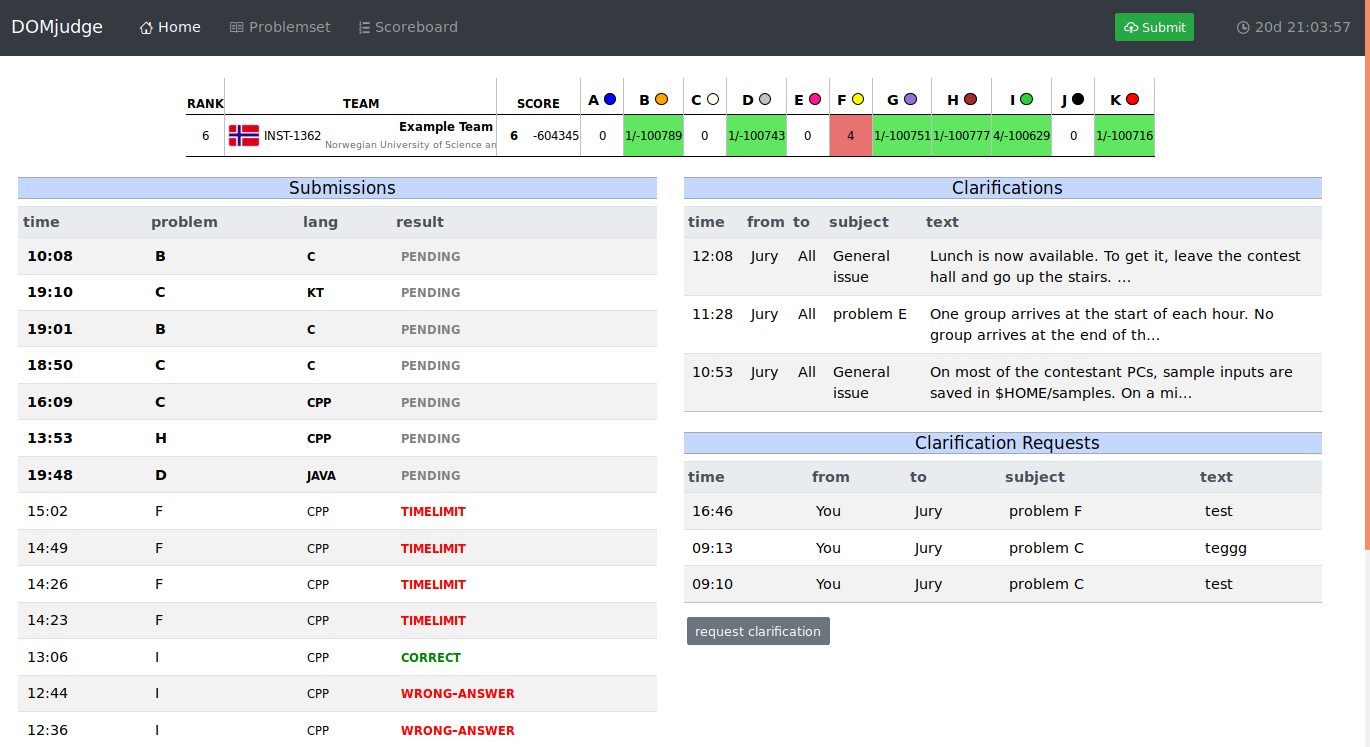
\includegraphics[width=\textwidth]{team-overview}}
  \caption{the team web interface overview page.}
  \label{fig:team-overview}
\end{figure}

\begin{figure}[p]
  \centering
  \fbox{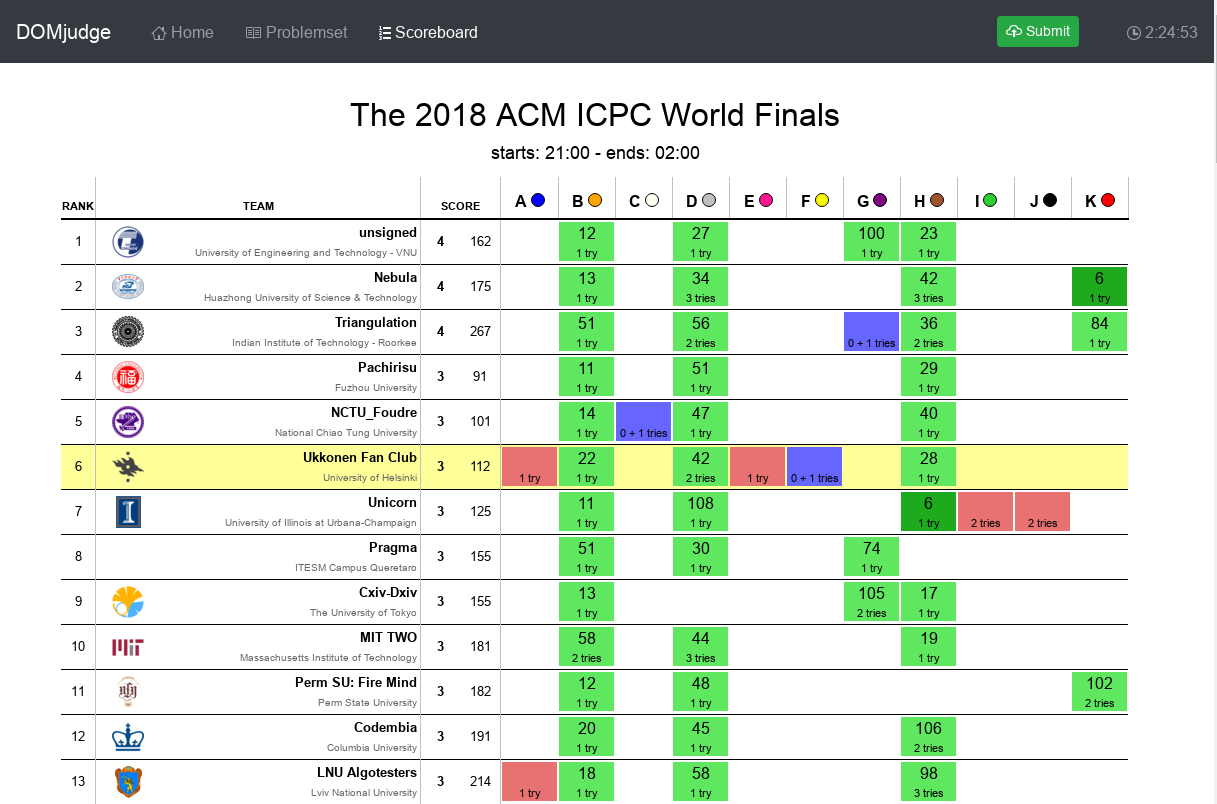
\includegraphics[width=\textwidth]{team-scoreboard}}
  \caption{the scoreboard webpage.}
  \label{fig:team-scoreboard}
\end{figure}

\newpage

\section{Submitting solutions}\label{submit}

\ifcmdsubmit{
Submitting solutions can be done in two ways: with the command-line
program \cmd{submit} or using the web interface. One of the
interfaces might not be available, depending on the system
configuration by the jury. A description of both methods follows.

\subsection{Command-line: \cmd{submit}}

\textbf{Syntax:} \cmd{submit [options] filename.ext ...}

The submit program takes the name (label) of the problem from
\cmd{filename} and the programming language from the extension
\cmd{ext}. This can be overruled with the options
\cmd{-p problemname} and \cmd{-l~languageextension}.
See \cmd{submit --help} for a complete list of all options,
extensions and some examples.  Use \cmd{submit~--help | more}
when the help text does not fit on one screen.

\cmd{submit} will check your file and warns you for some problems:
for example when the file has not been modified for a long time or
when it's larger than the maximum source code size.
Filenames must start with an alphanumerical character and may contain only
alphanumerical characters and \cmd{+.\_-}. You can specify multiple files
to be part of this submission (see section~\ref{howjudged} `How are
submissions being judged?').

Then \cmd{submit} displays a summary with all details of your
submission and asks for confirmation. Check whether you are submitting
the right file for the right problem and language and press `y' to
confirm. \cmd{submit} will report a successful submission or give
an error message otherwise.

The submit program uses a directory \cmd{\USERSUBMITDIR} in the
home directory of your account where it stores temporary files for
submission and also a log file \cmd{submit.log}. Do not remove or
change this directory, otherwise the \cmd{submit} program might fail to
function correctly.
}

\subsection{Web interface}

Solutions can be submitted from the web interface at \url{\BASEURL team}.
In the left column click the file selection button and select one or
multiple files for submission. \DOMjudge will try to determine the
problem and language from the base and extension of the (first) filename.
Otherwise, select the appropriate values.
Filenames must start with an alphanumerical character and may contain only
alphanumerical characters and \cmd{+.\_-}.

After you hit the submit button and confirm the submission, you will
be redirected back to your submission list page. On this page, a message
will be displayed that your submission was successful and the
submission should be present in the list. An error message will be
displayed if something went wrong.

\section{Viewing the results of submissions}

The left column of your team web page shows an overview of your submissions.
It contains all relevant information: submission time, programming
language, problem and status. The address of your team page is
\url{\BASEURL team}.

The top of the page shows your team's row in the scoreboard: your position and
which problems you attempted and solved. Via the menu you can view the public
scoreboard page with the scores of all teams. Many cells will show
additional ``title text'' information when hovering over them. The
score column lists the number of solved problems and the total penalty
time. Each cell in a problem column lists the number of submissions,
and if the problem was solved, the time of the first correct
submission in minutes since contest start. This is included in your
total time together with any penalty time incurred for previous
incorrect submissions. Optionally the scoreboard can
be `frozen' some time before the end of the contest. The full scoreboard view
will not be updated anymore, but your team row will. Your team's rank will
be displayed as `?'. Finally, via the top menu you can also view the
list of problems and view/download problem texts and sample data, if
provided by the jury.

\subsection{Possible results}

A submission can have the following results (not all of these may be
available depending on configuration of the system):

\begin{description}[\setleftmargin{4.5cm}]
\item[CORRECT]
The submission passed all tests: you solved this problem!

\item[COMPILER-ERROR]
There was an error when compiling your program. On the submission
details page you can inspect the exact error (this option might be
disabled).

\item[TIMELIMIT]
Your program took longer than the maximum allowed time for this
problem. Therefore it has been aborted. This might indicate that your
program hangs in a loop or that your solution is not efficient
enough.

\item[RUN-ERROR]
There was an error during the execution of your program. This can have
a lot of different causes like division by zero, incorrectly
addressing memory (e.g. by indexing arrays out of bounds), trying to
use more memory than the limit, etc.
Also check that your program exits with exit code 0!

\item[NO-OUTPUT]
Your program did not generate any output. Check that you write to
standard out.

\item[WRONG-ANSWER]
The output of your program was incorrect. This can happen simply
because your solution is not correct, but remember that your output
must comply exactly with the specifications of the jury.

\item[TOO-LATE]
Bummer, you submitted after the contest ended! Your submission is
stored but will not be processed anymore.
\end{description}

\section{Clarifications}

All communication with the jury is to be done through clarifications.
These can be found in the right column on your team page. Both
clarification replies from the jury and requests sent by you
are displayed there.

There is also a button to submit a new clarification request to the
jury; you can associate a specific problem or one of the general
categories to a request. This clarification request is only readable
for the jury. The jury can answer specifically to your team or send a
reply to everyone if it is relevant for all.

\section{How are submissions being judged?}\label{howjudged}

The \DOMjudge jury system is fully automated. In principle no human
interaction is necessary. The judging is done in the following way:

\subsection{Submitting solutions}

With%
\ifcmdsubmit{ the \cmd{submit} program or}
the web interface (see section~\ref{submit}) you can submit a solution
to a problem to the jury. Note that you have to submit the source code
of your program (and not a compiled program or the output of your
program).

On the jury system your program enters a queue, awaiting compilation,
execution and testing on one of the jury computers.

\subsection{Compilation}

Your program will be compiled on a jury computer running Linux.
All submitted source files will be passed to the compiler which
generates a single program to run; for languages where
this is relevant, the first file specified will be considered the
`main' source file.

Using a different compiler or operating system than the jury should
not be a problem. Be careful however, not to use any special compiler
and/or system specific things (you may be able to check compiler errors
on the team page).

The jury system defines \cmd{ONLINE\_JUDGE} and \cmd{DOMJUDGE}.
These are defined as preprocessor symbols in compiled languages and
as (environment) variables in scripted languages.

\subsection{Testing}

After your program has compiled successfully it will be executed and
its output compared to the output of the jury. Before comparing the
output, the exit status of your program is checked: if your program
gives the correct answer, but exits with a non-zero exit code, the
result will be a \textsc{run-error}! There are some restrictions during
execution. If your program violates these it will also be aborted
with a \textsc{run-error}, see section~\ref{runlimits}.

When comparing program output, it has to exactly match to output of
the jury, except that some extra whitespace may be ignored (this
depends on the jury's configuration of the problems). So take care
that you follow the output specifications. In case of problem
statements which do not have unique output (e.g. with floating point
answers), the jury may use a modified comparison function.

\subsection{Restrictions}\label{runlimits}

To prevent abuse, keep the jury system stable and give everyone
clear and equal environments, there are some restrictions to which all
submissions are subjected:

\begin{description}[\setlabelphantom{number of processes}]
\item[compile time]
Compilation of your program may take no longer than \COMPILETIME\
seconds. After that, compilation will be aborted and the result will
be a compile error. In practice this should never give rise to
problems. Should this happen to a normal program, please inform the
jury right away.

\item[source size]
The total amount of source code in a single submission may not exceed
\SOURCESIZE\ kilobytes, otherwise your submission will be rejected.

\item[memory]
During execution of your program, there are \MEMLIMIT\ kilobytes of
memory available. This is the total amount of memory (including
program code, statically and dynamically defined variables, stack,
Java VM, \dots)! If your program tries to use more memory, it will
abort, resulting in a run error.

\item[number of processes]
You are not supposed to create multiple processes (threads). This is
to no avail anyway, because your program has exactly 1 processor core fully
at its disposal. To increase stability of the jury system, there is a
maximum of \PROCLIMIT\ processes that can be run simultaneously
(including processes that started your program).

People who have never programmed with multiple processes (or have
never heard of ``threads'') do not have to worry: a normal program
runs in one process.

\end{description}

\subsection{Java class naming}

Compilation of Java sources is somewhat complicated by the class
naming conventions used: there is no fixed entry point; any class can
contain a method \texttt{main}. Furthermore, a class declared
\texttt{public} must be located in an indentically named file.

In the default configuration of DOMjudge this is worked around by
autodetecting the main class. When this feature is not used, then
the main class should be ``\verb!Main!'', with method
``\verb!public static void main(String args[])!'', see also the Java
code example in appendix~\ref{codeexamples}.

\newpage
\appendix

\section{Code examples}\label{codeexamples}

Below are a few examples on how to read input and write output for a
problem.

The examples are solutions for the following problem: the first line
of the input contains the number of testcases. Then each testcase
consists of a line containing a name (a single word) of at most 99
characters. For each testcase output the string ``Hello $<$name$>$!''
on a separate line.

Sample input and output for this problem:

\begin{tabular}{|p{0.47\textwidth}|p{0.47\textwidth}|}
\hline
\textbf{Input} & \textbf{Output} \\
\hline
\verbatiminput{../examples/example.in} &
\verbatiminput{../examples/example.out} \\
\hline
\end{tabular}

Note that the number 3 on the first line indicates that 3 testcases
follow.

A solution for this problem in C:
\listinginput{1}{../examples/example.c}

Notice the last \cmd{return 0;} to prevent a \textsc{run-error}!

\newpage

A solution in C++:
\listinginput{1}{../examples/example.cc}

A solution in Java:
\listinginput{1}{../examples/example.java}

\newpage

A solution in C\#:
\listinginput{1}{../examples/example.cs}

A solution in Pascal:
\listinginput{1}{../examples/example.pas}

And finally a solution in Haskell:
\listinginput{1}{../examples/example.hs}

\end{document}
